\documentclass{standalone}
\usepackage{tikz}
\usepackage{ctex,siunitx}
\setCJKmainfont{Noto Serif CJK SC}
\usepackage{tkz-euclide}
\usepackage{amsmath}
\usetikzlibrary{patterns, calc,3d}
\usetikzlibrary {decorations.pathmorphing,decorations.pathreplacing,decorations.shapes}
\tikzset{label style/.append style={font=\small}}
\begin{document}
\small
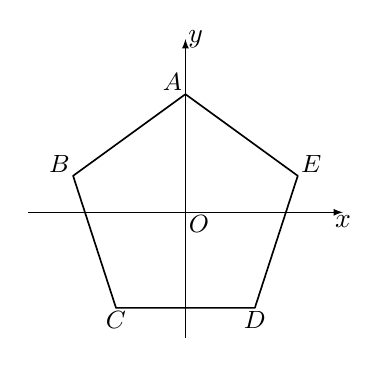
\begin{tikzpicture}[>=latex,scale=1.0,inner sep=1pt]
  \foreach \x[count=\i] in {A,B,C,D,E}
  { \tkzDefPoint({18+\i*72}:1.5){\x}}
  \tkzDefPoint(0,0){O}
  \draw[very thin,->](-2,0)--(2,0)node[below]{$x$};
  \draw[very thin,->](0,-1.6)--(0,2.2)node[right]{$y$};
  \tkzDrawPolygon[semithick](A,B,C,D,E)
  \tkzLabelPoints[below right](O)
  \tkzLabelPoints[above right](E)
  \tkzLabelPoints[above left](A,B)
  \tkzLabelPoints[below](D,C)
\end{tikzpicture}
\end{document}